\documentclass[conference,letterpaper]{IEEEtran}
\usepackage[T1]{fontenc}
\usepackage[utf8]{inputenc}
\usepackage{amsmath,amssymb}
\usepackage{graphicx}
\usepackage{cite}
\usepackage{url}
\usepackage{tikz}
\usetikzlibrary{arrows.meta,positioning,calc}

% Every measured number is a macro generated by paper/make_assets.py from results/*.csv.
\IfFileExists{generated/numbers.tex}{% Generated by paper/make_assets.py from results/*.csv. Do not edit by hand.
\providecommand{\notmeasured}{[not measured]}
\newcommand{\eEightApiCpuEval}{219}
\newcommand{\eEightApiCpuKeygen}{328}
\newcommand{\eEightApiWsEnd}{240.69}
\newcommand{\eEightPoliceCpuEval}{1,969}
\newcommand{\eEightPoliceCpuKeygen}{3,391}
\newcommand{\eEightPoliceWasm}{90.25}
\newcommand{\eEightPoliceWsEnd}{1040.56}
\newcommand{\eEightReps}{10}
\newcommand{\eEightUserCpuEval}{2,391}
\newcommand{\eEightUserCpuKeygen}{3,234}
\newcommand{\eEightUserWasm}{90.25}
\newcommand{\eEightUserWsEnd}{1005.19}
\newcommand{\eElevenBelow}{0}
\newcommand{\eElevenMaxP}{0.994}
\newcommand{\eElevenMinP}{0.219}
\newcommand{\eElevenRuns}{3,000}
\newcommand{\eElevenTests}{9}
\newcommand{\eFiveARuns}{304}
\newcommand{\eFiveBFifteenEach}{377}
\newcommand{\eFiveBFifteenM}{46}
\newcommand{\eFiveBFifteenOnce}{277}
\newcommand{\eFiveBFifteenPacked}{66.1}
\newcommand{\eFiveBMaxD}{32}
\newcommand{\eFiveBRuns}{30}
\newcommand{\eFiveBTotal}{1,530}
\newcommand{\eFiveBTwoEach}{50.9}
\newcommand{\eFiveBTwoM}{128}
\newcommand{\eFiveBTwoOnce}{44.1}
\newcommand{\eFiveBTwoPacked}{40.4}
\newcommand{\eFiveBWrong}{0}
\newcommand{\eFourBaseBudget}{272.4}
\newcommand{\eFourBaseClient}{44.2}
\newcommand{\eFourBaseCt}{1,536}
\newcommand{\eFourBaseMem}{99.12}
\newcommand{\eFourBaseServer}{91.5}
\newcommand{\eFourBestBudget}{7.5}
\newcommand{\eFourBestClient}{2.23}
\newcommand{\eFourBestCt}{64.3}
\newcommand{\eFourBestMem}{20.11}
\newcommand{\eFourBestN}{12}
\newcommand{\eFourBestP}{49}
\newcommand{\eFourBestQ}{60}
\newcommand{\eFourBestQP}{109}
\newcommand{\eFourBestServer}{2.94}
\newcommand{\eFourCorrect}{47}
\newcommand{\eFourFailList}{$\log N=15$, $\log Q=\{56\}$, uniform ternary secret (519 of 1011 runs wrong)}
\newcommand{\eFourIncorrect}{1}
\newcommand{\eFourInvalid}{0}
\newcommand{\eFourReps}{30}
\newcommand{\eFourRunsPerSet}{1011}
\newcommand{\eFourSets}{48}
\newcommand{\eFourShrinkCt}{24}
\newcommand{\eFourSparseCorrect}{24 of 24}
\newcommand{\eFourSparseRatio}{1.00}
\newcommand{\eFourSparseRatioMax}{1.39}
\newcommand{\eFourSparseRatioMin}{0.96}
\newcommand{\eFourSpeedClient}{20}
\newcommand{\eFourSpeedServer}{31}
\newcommand{\eFourTightBudget}{0.3}
\newcommand{\eFourWithin}{18}
\newcommand{\eNineAblateBgv}{11,974,817}
\newcommand{\eNineAblateBgvBr}{2.00}
\newcommand{\eNineAblateBgvGz}{2.76}
\newcommand{\eNineAblateBgvMiB}{11.42}
\newcommand{\eNineAblateEmptyRuntime}{1,964,129}
\newcommand{\eNineAblateEmptyRuntimeBr}{0.43}
\newcommand{\eNineAblateEmptyRuntimeGz}{0.56}
\newcommand{\eNineAblateEmptyRuntimeMiB}{1.87}
\newcommand{\eNineAblateGcOt}{3,058,834}
\newcommand{\eNineAblateGcOtBr}{0.63}
\newcommand{\eNineAblateGcOtGz}{0.83}
\newcommand{\eNineAblateGcOtMiB}{2.92}
\newcommand{\eNineAblateMpbgv}{11,957,145}
\newcommand{\eNineAblateMpbgvBr}{1.99}
\newcommand{\eNineAblateMpbgvGz}{2.76}
\newcommand{\eNineAblateMpbgvMiB}{11.40}
\newcommand{\eNineBrColdFetch}{89.0 [74.2, 102]}
\newcommand{\eNineBrColdReady}{141 [123, 155]}
\newcommand{\eNineBrColdTransfer}{11,526}
\newcommand{\eNineBrWarmFetch}{41.4 [36.9, 48.4]}
\newcommand{\eNineBrWarmReady}{94.3 [89.2, 102]}
\newcommand{\eNineBrWarmTransfer}{0}
\newcommand{\eNineBrWasmMem}{39.50}
\newcommand{\eNineLoadCompile}{14.0 [13.7, 14.2]}
\newcommand{\eNineLoadRead}{4.45 [4.29, 4.70]}
\newcommand{\eNineLoadRuns}{30}
\newcommand{\eNineLtPoliceCount}{6}
\newcommand{\eNineLtPoliceMax}{574}
\newcommand{\eNineLtPoliceTotal}{1,380}
\newcommand{\eNineLtUserCount}{6.5}
\newcommand{\eNineLtUserMax}{918}
\newcommand{\eNineLtUserTotal}{1,334}
\newcommand{\eNinePartyCommittedInRepo}{12,915,336}
\newcommand{\eNinePartyCommittedInRepoBr}{2.16}
\newcommand{\eNinePartyCommittedInRepoGz}{3.00}
\newcommand{\eNinePartyCommittedInRepoMiB}{12.32}
\newcommand{\eNinePartyDefault}{11,802,642}
\newcommand{\eNinePartyDefaultBr}{1.98}
\newcommand{\eNinePartyDefaultGz}{2.75}
\newcommand{\eNinePartyDefaultMiB}{11.26}
\newcommand{\eNinePartyDefaultWasmoptOz}{10,336,136}
\newcommand{\eNinePartyDefaultWasmoptOzBr}{1.95}
\newcommand{\eNinePartyDefaultWasmoptOzGz}{2.65}
\newcommand{\eNinePartyDefaultWasmoptOzMiB}{9.86}
\newcommand{\eNinePartyStrip}{11,488,036}
\newcommand{\eNinePartyStripBr}{1.94}
\newcommand{\eNinePartyStripGz}{2.69}
\newcommand{\eNinePartyStripMiB}{10.96}
\newcommand{\eNinePartyStripTrimpath}{11,443,013}
\newcommand{\eNinePartyStripTrimpathBr}{1.94}
\newcommand{\eNinePartyStripTrimpathGz}{2.69}
\newcommand{\eNinePartyStripTrimpathMiB}{10.91}
\newcommand{\eNinePartyStripWasmoptOz}{10,336,159}
\newcommand{\eNinePartyStripWasmoptOzBr}{1.95}
\newcommand{\eNinePartyStripWasmoptOzGz}{2.65}
\newcommand{\eNinePartyStripWasmoptOzMiB}{9.86}
\newcommand{\eNinePartyTrimpath}{11,757,642}
\newcommand{\eNinePartyTrimpathBr}{1.98}
\newcommand{\eNinePartyTrimpathGz}{2.75}
\newcommand{\eNinePartyTrimpathMiB}{11.21}
\newcommand{\eNineSlowETwos}{2.6}
\newcommand{\eNineSlowEncrypt}{2.7}
\newcommand{\eNineSlowEval}{2.7}
\newcommand{\eNineSlowGarble}{7.2}
\newcommand{\eNineSlowGcEval}{6.3}
\newcommand{\eNineSlowKeygen}{3.4}
\newcommand{\eNineSlowOt}{6.5}
\newcommand{\eNineSlowTotal}{3.4}
\newcommand{\eNineWasmRuns}{41}
\newcommand{\eOneBoundary}{9}
\newcommand{\eOneBrowserChrome}{Chrome 157.0.8103.52}
\newcommand{\eOneBrowserOk}{4}
\newcommand{\eOneBrowserRuns}{4}
\newcommand{\eOneFailed}{0}
\newcommand{\eOneFixed}{11}
\newcommand{\eOneInside}{4,760}
\newcommand{\eOneMismatch}{0}
\newcommand{\eOneOutside}{5,242}
\newcommand{\eOneRandom}{10,000}
\newcommand{\eOneRuns}{10,011}
\newcommand{\eSevenClientUp}{18,776}
\newcommand{\eSevenGC}{8.75}
\newcommand{\eSevenTrPoliceDown}{25,606}
\newcommand{\eSevenTrPolicePoll}{35}
\newcommand{\eSevenTrPoliceRequests}{64}
\newcommand{\eSevenTrPoliceUp}{18,777}
\newcommand{\eSevenTrPoliceWasm}{11,526}
\newcommand{\eSevenTrReps}{5}
\newcommand{\eSevenTrUserDown}{25,622}
\newcommand{\eSevenTrUserPoll}{35}
\newcommand{\eSevenTrUserRequests}{63}
\newcommand{\eSevenTrUserUp}{18,784}
\newcommand{\eSevenTrUserWasm}{11,526}
\newcommand{\eSixBestN}{20}
\newcommand{\eSixBestThroughput}{39.6}
\newcommand{\eSixBrChrome}{Chrome 157.0.8103.52}
\newcommand{\eSixBrConcurrentOneOne}{8.89}
\newcommand{\eSixBrConcurrentOneOneIQR}{[8.88, 8.90]}
\newcommand{\eSixBrConcurrentOneThree}{15.11}
\newcommand{\eSixBrConcurrentOneThreeIQR}{[15.04, 15.23]}
\newcommand{\eSixBrConcurrentOneTwo}{12.08}
\newcommand{\eSixBrConcurrentOneTwoIQR}{[11.87, 12.15]}
\newcommand{\eSixBrConcurrentThreeOne}{8.17}
\newcommand{\eSixBrConcurrentThreeOneIQR}{[8.14, 8.42]}
\newcommand{\eSixBrConcurrentThreeThree}{16.42}
\newcommand{\eSixBrConcurrentThreeThreeIQR}{[15.62, 16.43]}
\newcommand{\eSixBrConcurrentThreeTwo}{12.13}
\newcommand{\eSixBrConcurrentThreeTwoIQR}{[12.12, 12.13]}
\newcommand{\eSixBrConcurrentTwoOne}{11.88}
\newcommand{\eSixBrConcurrentTwoOneIQR}{[11.84, 11.97]}
\newcommand{\eSixBrConcurrentTwoThree}{13.06}
\newcommand{\eSixBrConcurrentTwoThreeIQR}{[12.29, 17.65]}
\newcommand{\eSixBrConcurrentTwoTwo}{19.20}
\newcommand{\eSixBrConcurrentTwoTwoIQR}{[19.19, 19.21]}
\newcommand{\eSixBrFailed}{2}
\newcommand{\eSixBrInputResult}{3.45 [3.45, 3.48]}
\newcommand{\eSixBrReps}{5}
\newcommand{\eSixBrRows}{210}
\newcommand{\eSixBrSequentialOneOne}{6.87}
\newcommand{\eSixBrSequentialOneOneIQR}{[6.85, 6.88]}
\newcommand{\eSixBrSequentialThreeOne}{17.83}
\newcommand{\eSixBrSequentialThreeOneIQR}{[16.83, 17.85]}
\newcommand{\eSixBrSequentialTwoOne}{11.84}
\newcommand{\eSixBrSequentialTwoOneIQR}{[11.83, 12.83]}
\newcommand{\eSixBrSetup}{2.54 [2.51, 2.86]}
\newcommand{\eSixBrTotal}{8.88 [8.88, 8.90]}
\newcommand{\eSixCrashed}{0}
\newcommand{\eSixFailedPairs}{0}
\newcommand{\eSixLatencyOne}{165 [163, 166]}
\newcommand{\eSixLatencyThree}{185 [182, 188]}
\newcommand{\eSixMaxMem}{6,137}
\newcommand{\eSixMaxPairs}{128}
\newcommand{\eSixMaxUtil}{88}
\newcommand{\eSixMemPerPair}{43.5}
\newcommand{\eSixRamLimit}{360}
\newcommand{\eSixReps}{5}
\newcommand{\eSixSeqThroughput}{6.12}
\newcommand{\eTenClassHoursFive}{0}
\newcommand{\eTenClassHoursOne}{4}
\newcommand{\eTenClassHoursTwo}{2}
\newcommand{\eTenClassIQR}{[12, 13]}
\newcommand{\eTenClassMax}{14}
\newcommand{\eTenClassMedian}{13}
\newcommand{\eTenClassMin}{4}
\newcommand{\eTenExactHoursFive}{0}
\newcommand{\eTenExactHoursOne}{0}
\newcommand{\eTenExactHoursTwo}{0}
\newcommand{\eTenExactIQR}{[2, 2]}
\newcommand{\eTenExactMax}{2}
\newcommand{\eTenExactMedian}{2}
\newcommand{\eTenExactMin}{1}
\newcommand{\eTenPoints}{300}
\newcommand{\eThirteenOk}{4}
\newcommand{\eThirteenRuns}{4}
\newcommand{\eThreeBudget}{272.6}
\newcommand{\eThreeBudgetMin}{272.2}
\newcommand{\eThreeDelta}{54.4}
\newcommand{\eThreeDeltaMax}{54.8}
\newcommand{\eThreeETwos}{7.08}
\newcommand{\eThreeEncrypt}{30.9}
\newcommand{\eThreeEval}{52.9}
\newcommand{\eThreeFailed}{0}
\newcommand{\eThreeFlood}{$-$6.3}
\newcommand{\eThreeFloodMax}{$-$6.3}
\newcommand{\eThreeFresh}{23.5}
\newcommand{\eThreeGarble}{0.0601}
\newcommand{\eThreeGarbled}{5,322}
\newcommand{\eThreeGcEval}{0.0111}
\newcommand{\eThreeKeygen}{67.0}
\newcommand{\eThreeMismatch}{0}
\newcommand{\eThreeNoiseStd}{36.3}
\newcommand{\eThreeOt}{1.99}
\newcommand{\eThreeQBits}{328}
\newcommand{\eThreeRuns}{1,011}
\newcommand{\eThreeTotal}{145 [143, 147]}
\newcommand{\eTwoFailed}{0}
\newcommand{\eTwoFirstWrongNeg}{$-$32,769}
\newcommand{\eTwoFirstWrongPos}{32,769}
\newcommand{\eTwoLastGoodNeg}{$-$32,768}
\newcommand{\eTwoLastGoodPos}{32,768}
\newcommand{\eTwoRuns}{239}
\newcommand{\eTwoWrong}{114}
\newcommand{\hwAC}{AC power}
\newcommand{\hwCPU}{13th Gen Intel Core i9-13900H}
\newcommand{\hwCommit}{2fd5a89}
\newcommand{\hwCores}{14}
\newcommand{\hwDate}{2026-11-12}
\newcommand{\hwDefender}{enabled}
\newcommand{\hwGo}{go1.26.0}
\newcommand{\hwModel}{HUAWEI MCLG-XX}
\newcommand{\hwNode}{v22.21.0}
\newcommand{\hwOS}{Microsoft Windows 11 Home Single Language (10.0.26300)}
\newcommand{\hwPower}{Equilibrado}
\newcommand{\hwRAM}{15.7}
\newcommand{\hwThreads}{20}
}{}
\newcommand{\num}[1]{\ifcsname #1\endcsname\csname #1\endcsname\else\textbf{[not measured]}\fi}
\newcommand{\tabwide}[1]{\IfFileExists{generated/#1}{\input{generated/#1}}{\textbf{[not measured]}}}
\newcommand{\tabin}[1]{\IfFileExists{generated/#1}{\resizebox{\ifdim\width>\columnwidth\columnwidth\else\width\fi}{!}{\input{generated/#1}}}{\textbf{[not measured]}}}
\newcommand{\figin}[2][\columnwidth]{\IfFileExists{generated/#2}{\includegraphics[width=#1]{generated/#2}}{\fbox{\textbf{[figure not generated: \detokenize{#2}]}}}}
\newcommand{\todo}[1]{\textbf{[#1]}}
\renewcommand{\arraystretch}{1.15}

\begin{document}

\title{Private Proximity: Multiparty Homomorphic Encryption with Garbled Circuits}

\author{\IEEEauthorblockN{Carlos Eduardo Arias Capetillo, Alberto L\'opez Barrag\'an, Fernanda Santill\'an Dant\'es}
\IEEEauthorblockA{Instituto Tecnol\'ogico y de Estudios Superiores de Monterrey, Campus Monterrey\\
Av. Eugenio Garza Sada 2501, Col. Tecnol\'ogico, C.P. 64700, Monterrey, Nuevo Le\'on, Mexico\\
Advisor: Juan David Guarnizo Hernandez}}
\maketitle

\begin{abstract}
Private Proximity is a browser-based prototype in which a Police client and a User client decide whether the User's location is inside, outside, or exactly on the boundary of a public radius around a reference point, without either side revealing its coordinates. An earlier version decrypted the margin $\Delta = \text{dist}^2 - R^2$, which gave the Police the exact distance. The version evaluated here never decrypts $\Delta$: a two-party BGV computation produces $\mathrm{Enc}(\Delta)$, an encryption-to-shares step turns it into additive shares modulo $t = 65{,}537$, and a Yao garbled circuit with oblivious transfer outputs only the class. We measured the cryptographic pipeline natively on one laptop. All \num{eOneRuns} end-to-end runs of the correctness experiment matched a plaintext oracle. The class is correct for every $\Delta$ from \num{eTwoLastGoodNeg} to \num{eTwoLastGoodPos} and wrong immediately outside that range. With the deployed parameters ($N = 2^{14}$, $\log QP = 438$) only about \num{eThreeDelta} of the \num{eThreeQBits} ciphertext-modulus bits are consumed, and a parameter sweep found a correct set at $N = 2^{\num{eFourBestN}}$ with $\log QP = \num{eFourBestQP}$ that lowers one client's work by a factor of \num{eFourSpeedClient} and the server's by \num{eFourSpeedServer}. We also report two limits: the noise-flooding term of the share conversion is smaller than the ciphertext noise it is meant to hide, and a garbler that deviates from the protocol can recover $\Delta$ in 17 executions, so the semi-honest assumption is essential. Browser-level latency, HTTP traffic and robustness experiments were not run and are listed as open.
\end{abstract}

\begin{IEEEkeywords}
secure multiparty computation, homomorphic encryption, garbled circuits, oblivious transfer, location privacy, WebAssembly
\end{IEEEkeywords}

\section{Introduction}
Location is among the most sensitive data a person produces, and proximity questions (``was this person near that place?'') are often answered by handing a full location history to whoever asks. Secure computation offers a narrower alternative: two parties compute an agreed function of their private inputs and learn only its output.

\textbf{Context.} Private Proximity simulates a police inquiry. The Police hold a reference point $P$ (a case scene) and a public radius $R$; a User holds a private location $U$. Both run a WebAssembly client in the browser, and a Go server coordinates the protocol and evaluates encrypted arithmetic.

\textbf{Problem.} In the previous version of the prototype the Police decrypted $\Delta = \text{dist}^2 - R^2$. That value reveals the exact distance to the User, and a few queries with different reference points are enough to locate the User.

\textbf{Justification.} The question posed by the scenario has three possible answers. Revealing only that answer discloses strictly less than the distance, and it lets us study what such a design costs in a browser deployment.

\textbf{Objective.} Replace the plaintext decryption of $\Delta$ with a garbled circuit that reveals only the classification, and evaluate the result: correctness against a plaintext reference, the limits of the encoding, the cost per participant, and what the remaining leakage is.

\textbf{Hypothesis.} For inputs inside the supported range and parties that follow the protocol, the encrypted workflow returns the same class as a plaintext computation, and the Police obtain no more than that class from one evaluation.

The research question addressed in this work is:
\begin{quote}
\itshape \todo{RESEARCH QUESTION: the project's existing wording must be inserted here by the authors. It was not available when this draft was generated and has deliberately not been paraphrased.}
\end{quote}

\section{Background}
\subsection{BGV Homomorphic Encryption}
BGV~\cite{bgv} is a leveled homomorphic encryption scheme based on the ring learning-with-errors problem. Let $R = \mathbb{Z}[X]/(X^N+1)$ with $N$ a power of two, $R_Q = R/QR$ for a ciphertext modulus $Q$, and $t$ a plaintext modulus. The secret key is a polynomial $s \in R$ with small coefficients. A ciphertext is a pair $(c_0, c_1) \in R_Q^2$ such that
\begin{equation}
c_0 + c_1 s \equiv m + t e \pmod{Q},
\label{eq:bgv}
\end{equation}
where $m \in R_t$ is the message and $e$ is a small noise polynomial. Decryption computes the left-hand side, takes the centered representative modulo $Q$ and reduces it modulo $t$; it is correct as long as $\lVert m + te \rVert_\infty < Q/2$. (Lattigo stores an equivalent form in which the message is multiplied by $t^{-1} \bmod Q$; the correctness condition is the same.)

Ciphertexts are added componentwise, and the noises add. Multiplying two ciphertexts yields three components that decrypt under $(1, s, s^2)$ and multiplies the noise terms; a \emph{relinearization key}, an encryption of $s^2$ over an auxiliary modulus $P$, brings the result back to two components. Each multiplication therefore consumes part of the \emph{noise budget} $\log_2(Q/2) - \log_2 \lVert m + te \rVert_\infty$, which is why $Q$ is chosen from the multiplicative depth of the function. When $t \equiv 1 \pmod{2N}$, $R_t$ splits into $N$ slots that are added and multiplied independently. Security rests on the size of $N$ relative to $\log_2 QP$: a larger modulus needs a larger ring.

\subsection{Multiparty BGV}
In the multiparty construction of Mouchet et al.~\cite{mouchet}, party $i$ holds a share $s_i$ and the collective secret key is $s = \sum_i s_i$, which is never assembled. For the \emph{collective public key} (CPK), all parties use the same public random polynomial $a$, derived from a common reference string; each publishes $p_i = -a s_i + e_i$, and the key is $(\sum_i p_i,\ a)$. The \emph{relinearization key} (RLK) is produced by a similar protocol with two rounds. Anyone holding these public keys can encrypt and evaluate; decryption needs a contribution from every party. With two parties, neither can decrypt alone, and the server, which holds no share, cannot decrypt at all. The prototype uses the implementation in Lattigo~v6.2.0~\cite{lattigo}.

\subsection{Encryption-to-Shares}
Encryption-to-shares (E2S)~\cite{mouchet} replaces decryption when the plaintext itself must stay hidden. For a ciphertext $(c_0, c_1)$, party $i$ samples a uniform mask $M_i \in R_t$ and publishes
\begin{equation}
h_i = c_1 s_i + e'_i - M_i ,
\label{eq:e2s}
\end{equation}
with $M_i$ encoded in $R_Q$ and $e'_i$ a fresh \emph{flooding} noise, drawn much wider than the encryption noise so that it hides the noise already in the ciphertext. Anyone can add the public shares to $c_0$ and decode $m - \sum_i M_i$, a value that is uniformly distributed. One designated party adds its own mask back. With two parties, the Police keep $s_P = M_P$ and the User obtains $s_U = m - M_P$, so that for the margin $\Delta$ of Section~\ref{sec:model}
\begin{equation}
s_P + s_U \equiv \Delta \pmod{t},
\label{eq:shares}
\end{equation}
and each share alone is uniform.

\subsection{Yao Garbled Circuits}
A garbled circuit~\cite{yao,bhr} lets an \emph{evaluator} compute a Boolean circuit on inputs it cannot read. The \emph{garbler} assigns two random 128-bit labels to every wire, one for each bit value. The evaluator holds exactly one label per wire and cannot tell which value it stands for. With the free-XOR technique~\cite{freexor}, the two labels of every wire differ by the same secret offset, so the label of an XOR output is the XOR of the input labels and needs no ciphertext; NOT gates are also free. For each AND gate the garbler sends four ciphertexts, each encrypting the correct output label under one combination of input labels, here with SHA-256 as the key-derivation function. Point-and-permute~\cite{bmr} stores one pointer bit in every label so that the evaluator decrypts only the row that corresponds to the labels it holds. One \emph{decode bit} per output wire turns the final labels into output bits. The cost of a circuit is thus its number of AND gates.

The circuit used here takes the two 17-bit shares, adds them modulo $t$ with a ripple-carry adder and outputs two bits: whether the centered result is negative and whether it is zero.

\subsection{Oblivious Transfer}
The evaluator needs the labels of its own input bits, but the garbler must not learn those bits and the evaluator must not obtain both labels of any wire. This is 1-out-of-2 oblivious transfer (OT): a sender holds $(m_0, m_1)$, a receiver holds a bit $b$ and learns only $m_b$. The implementation follows the protocol of Chou and Orlandi~\cite{chou} over the edwards25519 group with base point $B$: the sender publishes $A = aB$; for each bit the receiver publishes $R = xB + bA$; the sender encrypts $m_0$ under a key derived from $aR$ and $m_1$ under a key derived from $a(R - A)$; the receiver can derive only the key from $xA$. The three messages are named \texttt{otA}, \texttt{otR} and \texttt{otE} in the prototype, and one run transfers the 17 labels of the Police share.
\section{Architecture and System Model}
\label{sec:model}

\subsection{Actors and Trust Boundaries}
One \emph{assignment} involves three actors (Fig.~\ref{fig:arch}). The \emph{Police client} holds $P = (P_x, P_y)$ and a share of the secret key. The \emph{User client} holds $U = (U_x, U_y)$ and the other share. The \emph{server} (Go API with SQLite) holds no key share: it aggregates public shares, evaluates the encrypted arithmetic and relays the circuit messages. Secret keys, coordinates and additive shares never leave the browser that created them. All parties are assumed semi-honest: they follow the protocol but inspect what they receive.

\begin{figure}[t]
\centering
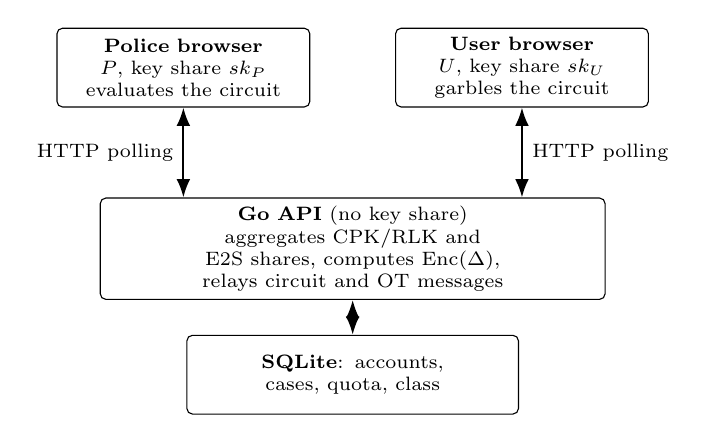
\begin{tikzpicture}[font=\scriptsize,
  box/.style={draw, rounded corners=2pt, align=center, minimum height=10mm, inner sep=3pt},
  arr/.style={Latex-Latex, thick}]
\node[box, text width=30mm] (police) at (-2.15,0) {\textbf{Police browser}\\$P$, key share $sk_P$\\evaluates the circuit};
\node[box, text width=30mm] (user) at (2.15,0) {\textbf{User browser}\\$U$, key share $sk_U$\\garbles the circuit};
\node[box, text width=62mm] (api) at (0,-2.3) {\textbf{Go API} (no key share)\\aggregates CPK/RLK and E2S shares, computes $\mathrm{Enc}(\Delta)$,\\relays circuit and OT messages};
\node[box, text width=40mm] (db) at (0,-3.9) {\textbf{SQLite}: accounts, cases, quota, class};
\draw[arr] (police.south) -- node[left]{HTTP polling} (police.south |- api.north);
\draw[arr] (user.south) -- node[right]{HTTP polling} (user.south |- api.north);
\draw[arr] (api) -- (db);
\end{tikzpicture}
\caption{Actors and communication in one assignment. Each browser box is a trust boundary: plaintext coordinates, secret-key shares and additive shares of $\Delta$ never leave it; only public shares, ciphertexts and garbled material travel over HTTP.}
\label{fig:arch}
\end{figure}

\subsection{Computed Function}
With public radius $R$, the server evaluates under the collective key
\begin{equation}
\Delta = (P_x - U_x)^2 + (P_y - U_y)^2 - R^2 ,
\label{eq:delta}
\end{equation}
which needs multiplicative depth one. Throughout this paper $\Delta$ denotes this margin. (The global offset of the free-XOR technique, also called ``delta'' in the garbling literature, is referred to as the \emph{free-XOR offset}.) Coordinates and radius are integers in $[0, 100]$, hence $\Delta \in [-10{,}000,\ 20{,}000]$.

\subsection{Protocol Steps}
(1)~Both clients generate key shares and contribute to the CPK and to the two RLK rounds. (2)~Each client encrypts its two coordinates under the CPK, one ciphertext per coordinate, using slot~0 only. (3)~The server computes $\mathrm{Enc}(\Delta)$ by~\eqref{eq:delta}. (4)~Both clients run E2S with discrete Gaussian flooding noise of standard deviation $2^{30}$ and obtain shares satisfying~\eqref{eq:shares}. (5)~The User garbles a circuit that adds the two 17-bit shares modulo $t$ and outputs two bits, $[\Delta < 0,\ \Delta = 0]$; the Police obtain their input labels by oblivious transfer, evaluate the circuit and learn only the class: \emph{inside}, \emph{boundary} or \emph{outside}.

\section{Implementation Details}
\subsection{Server}
The server is a Go program with an SQLite database. It authenticates clients with per-tab bearer tokens, stores accounts, cases, assignments, the evaluation quota and the final class, and exposes the endpoints that carry setup shares, ciphertexts, E2S shares and the five circuit messages (garbled tables, garbler labels, \texttt{otA}, \texttt{otR}, \texttt{otE}). The endpoints of the earlier version that returned a decryption of $\Delta$ were removed.

\subsection{WebAssembly Client}
The cryptographic client is the same Go code compiled with \texttt{GOOS=js GOARCH=wasm}. JavaScript loads the module and calls it through a single JSON entry point; a one-second timer polls the server and advances the protocol, with a guard against overlapping rounds.

\subsection{State Recovery}
Each client serializes its local cryptographic state (key share, E2S mask, garbling secrets) to IndexedDB, keyed by session and role, before it publishes the corresponding public message. A reload therefore resumes the same session instead of creating a second key share. If the local state is lost, either party can reset the session, which discards all public material of that pair.

\subsection{Quota}
The server allows one evaluation per assignment and three evaluations per Police--User pair per hour. The experiments below never change this limit; they run the cryptographic pipeline natively, outside the server.

\section{Security Discussion}
\subsection{Model and What Is Protected}
Under the semi-honest model, the server sees public key-generation shares, ciphertexts, public E2S shares and garbled material; the User sees no output; the Police see two output bits. The design does not protect against a party that deviates from the protocol, against a server that distributes modified client code, or against repeated queries.

\subsection{Server's View of the Share Conversion (E11)}
The only plaintext-domain value the server can derive is $c_0$ plus the aggregated public E2S share, which equals $\Delta$ minus both masks. We sampled it in \num{eElevenRuns} runs for three fixed inputs (Table~\ref{tab:e11}). Of \num{eElevenTests} chi-square tests, \num{eElevenBelow} had $p < 0.01$ (smallest $p = \num{eElevenMinP}$, largest $p = \num{eElevenMaxP}$): the samples are consistent with a uniform distribution and with a distribution that does not depend on the class. This is a sanity check of the implementation, not a proof; uniformity follows from the uniform masks by construction. A text search of the server source (\texttt{results/e11\_route\_audit.md}) found 22 API routes whose JSON fields carry only ciphertexts, public shares, garbled material, status flags and the final class, and no use of a decryptor or secret key in the server package. Handler bodies were not reviewed line by line, and no database, log or HTTP capture was scanned.

\begin{table}[t]
\caption{Chi-square tests on the server's view of E2S ($p$ from the Wilson--Hilferty approximation).}
\label{tab:e11}
\centering\scriptsize
\tabin{tab_e11.tex}
\end{table}

\subsection{Flooding Margin (E3)}
E2S hides the ciphertext noise behind fresh ``flooding'' noise. We measured the noise of $\mathrm{Enc}(\Delta)$ after the multiplication: its standard deviation is about $2^{\num{eThreeNoiseStd}}$, whereas the flooding noise has standard deviation $2^{30}$. The flooding term is therefore \emph{smaller} than the noise it should mask, by a median of \num{eThreeFlood} bits (largest value over all runs: \num{eThreeFloodMax}). Correctness is unaffected, but the statistical argument that the public E2S shares leak nothing about the secret keys or the inputs through the noise does not hold with this margin. We report it as an open issue: the definition of the margin is ours, and the consequence should be confirmed before any stronger claim. A larger flooding parameter is affordable, since \num{eThreeBudget} bits of noise budget remain unused.

\subsection{Repeated Queries (E10)}
We simulated an attacker who controls the Police point and the radius and wants to locate a hidden User on the $101 \times 101$ grid (\num{eTenPoints} random hidden points). With the old protocol, which revealed $\Delta$, the median attacker needs \num{eTenExactMedian} queries (maximum \num{eTenExactMax}). With classification only, an adaptive attacker that greedily halves the candidate set needs a median of \num{eTenClassMedian} queries (IQR \num{eTenClassIQR}, range \num{eTenClassMin}--\num{eTenClassMax}; Fig.~\ref{fig:e10}), close to the information bound of $\log_2 10{,}201 \approx 13.3$ bits. Under the quota of three evaluations per hour this takes a median waiting time of \num{eTenClassHoursOne}~h for one Police account. The quota is keyed by Police--User pair, so colluding accounts divide that time: \num{eTenClassHoursTwo}~h with two accounts and \num{eTenClassHoursFive}~h with five. The quota slows the attack; it does not prevent it.

\begin{figure}[t]
\centering
\figin{fig_e10_queries.pdf}
\caption{Queries an adaptive attacker needs to isolate a hidden grid point when each query returns only the class (simulation, no cryptography). The dashed line is $\log_2 10{,}201$. Most points fall within a few queries of the bound because a circle splits the candidate set almost evenly.}
\label{fig:e10}
\end{figure}

\subsection{Cheating Garbler (E12)}
The evaluator cannot check that a garbled AND table encodes AND. In a unit test that is not part of the application, a garbler that rewrites the 16 AND gates of the ``$\Delta = 0$'' chain makes the second output bit equal one chosen bit of $\Delta \bmod t$; 17 such garblings recovered $\Delta \bmod t$ exactly in 300 of 300 trials, and the evaluator reported no error. A second test forces the output ``outside'' for every input by altering the decode bits. With the roles of the prototype (the User garbles) this is an integrity failure: a dishonest User chooses the class the Police see. The first test shows that the function being computed is whatever the garbler decides, which is why the semi-honest assumption cannot be dropped without adding protection against malicious garblers.

\subsection{Out-of-Range Inputs (E2)}
The server cannot see whether an encrypted coordinate is in $[0, 100]$. Section~\ref{sec:e2} shows that an input that pushes $\Delta$ beyond $\pm 32{,}768$ flips the class, so a modified client can force a wrong result without being detected.

\subsection{Human in the Loop}
A query is created by an authenticated Police account, and nothing is computed until the User opens the request and presses the button that encrypts and submits the location; the User's interface states that the result goes only to the Police. Consent is therefore per assignment and explicit. What the User cannot verify is the Police point or the purpose of the query, and the User is not told the outcome. Who is entitled to open a case, and how that authorization is audited, is outside the prototype.

\section{Experimental Evaluation}
\label{sec:eval}
\subsection{Setup and Method}
All measurements were taken on one laptop: \num{hwModel}, \num{hwCPU} (\num{hwCores} cores, \num{hwThreads} threads), \num{hwRAM}~GiB RAM, \num{hwOS}, \num{hwGo}, commit \texttt{\num{hwCommit}}, on \num{hwDate}. The experiments drive the application's own packages from a native Go harness; the HTTP server, SQLite and the browser are not in the loop unless stated. Each experiment writes one CSV row per run; tables report medians with the interquartile range. Three warm-up runs are discarded. Time is read from the Windows performance counter because Go's monotonic clock on Windows returned 0 for sub-millisecond phases. Memory figures are peak working set, the Windows counterpart of resident set size.

\emph{Deviations from the planned protocol.} The Windows power plan was ``\num{hwPower}'' (Balanced) rather than best performance, and Windows Defender real-time protection was \num{hwDefender}. E1--E3 were started on battery; the machine entered standby during the first E2 run, which was kept as a raw file and repeated. Random inputs and the common reference string are seeded; Lattigo's key and encryption randomness cannot be seeded. Parameter sets were timed with \num{eFourReps} repetitions. The first passes of E4 and E5a overlapped with compilation jobs on the same machine and showed inflated times, so both were repeated on an idle machine; the first-pass files are kept in \texttt{results/raw/}. The first pass of E5b failed in the packed variant for dimensions that are not powers of two because of an error in the harness (the inner sum needs a power-of-two width); it was corrected and E5b was repeated.

\subsection{Correctness (E1)}
\num{eOneRuns} evaluations (\num{eOneFixed} named cases, Table~\ref{tab:e1}, and \num{eOneRandom} uniformly random inputs in $[0,100]$) were compared with the plaintext class: \num{eOneMismatch} mismatches and \num{eOneFailed} failed runs. The observed classes were \num{eOneInside} inside, \num{eOneBoundary} boundary and \num{eOneOutside} outside. The same check was made end to end in the browser: four scenarios with $P=(10,20)$ and $R=5$ were driven in headless \num{eOneBrowserChrome} against the real server and WebAssembly client, and \num{eOneBrowserOk} of \num{eOneBrowserRuns} showed the expected page (inside, boundary, outside, and the quota error on a fourth evaluation of the same pair within one hour; Appendix~A).

\begin{table}[t]
\caption{Named correctness cases (E1).}
\label{tab:e1}
\centering\scriptsize
\tabin{tab_e1.tex}
\end{table}

\subsection{Sign-Wrap Limit (E2)}
\label{sec:e2}
Bypassing the client's input check, we swept the true $\Delta$ from $-70{,}000$ to $70{,}000$ and every integer near $\pm 32{,}768$ (\num{eTwoRuns} runs, \num{eTwoFailed} failed). The class is correct for $\Delta$ from \num{eTwoLastGoodNeg} to \num{eTwoLastGoodPos}; the first wrong results are at \num{eTwoFirstWrongNeg} and \num{eTwoFirstWrongPos} (Fig.~\ref{fig:e2}). The reason is the centered representation modulo $t = 65{,}537$: values wrap to the opposite sign. Beyond $\pm 65{,}537$ the value wraps a full turn and the class is right again by coincidence.

\begin{figure}[t]
\centering
\figin{fig_e2_wrap.pdf}
\caption{Value compared by the circuit against the true $\Delta$ (integers, no unit). Dashed lines mark $\pm 32{,}768$. Outside them the decoded value has the opposite sign, so the class is wrong; the application's range $[-10{,}000, 20{,}000]$ lies well inside.}
\label{fig:e2}
\end{figure}

\subsection{Noise and Phase Times (E3)}
In \num{eThreeRuns} runs with fresh keys every 50 runs there were \num{eThreeMismatch} mismatches and \num{eThreeFailed} failures. A fresh ciphertext carries $|m + te|$ of about $2^{\num{eThreeFresh}}$; after the multiplication this grows to $2^{\num{eThreeDelta}}$ (maximum $2^{\num{eThreeDeltaMax}}$), against a modulus of \num{eThreeQBits} bits. The remaining budget after E2S is \num{eThreeBudget} bits (minimum \num{eThreeBudgetMin}). The chain is far larger than a depth-one computation needs, which motivates the sweep in Section~\ref{sec:e4}. Table~\ref{tab:e3} gives the time per phase: the lattice operations dominate, and the garbled circuit (\num{eThreeGarbled} bytes) costs microseconds because it has few AND gates; within the circuit phase the 17 oblivious transfers dominate.

\begin{table}[t]
\caption{Native time per phase in ms, deployed parameters (E3, both parties' work summed where applicable).}
\label{tab:e3}
\centering\scriptsize
\tabin{tab_e3.tex}
\end{table}

\subsection{Parameter Sweep (E4)}
\label{sec:e4}
We tested \num{eFourSets} parameter sets: $\log N \in \{12,\dots,15\}$, six modulus chains from 109 to 438 bits, and two secret-key distributions (Lattigo's default uniform ternary, and ternary with Hamming weight 192). Each set ran in its own process with \num{eFourReps} timed repetitions and \num{eFourRunsPerSet} correctness runs. \num{eFourCorrect} sets were correct in every run, \num{eFourIncorrect} were not, and \num{eFourInvalid} could not be instantiated. Table~\ref{tab:e4} lists the default-secret sets.

\emph{Security check.} ``Std.'' compares $\log QP$ with the largest modulus that the Homomorphic Encryption Standard~\cite{hestd} lists for 128-bit classical security with a uniform ternary secret (109, 218, 438 and 881 bits for $N = 2^{12}$ to $2^{15}$). The deployed set sits exactly on that bound. This is a lookup in a 2018 table, not a current estimator run, and it does not cover the multiparty setting or sparse secrets; we therefore do not state a security level for any set, only whether it is within that table.

The fastest set that is both correct and within the table is $\log N = \num{eFourBestN}$, $\log Q = \{\num{eFourBestQ}\}$, $\log P = \{\num{eFourBestP}\}$: one client's total work (key generation shares, encryption, E2S share) is \num{eFourBestClient}~ms against \num{eFourBaseClient}~ms for the deployed set (\num{eFourSpeedClient}$\times$), the server's is \num{eFourBestServer}~ms against \num{eFourBaseServer}~ms (\num{eFourSpeedServer}$\times$), and a ciphertext shrinks from \num{eFourBaseCt} to \num{eFourBestCt}~KiB. Its smallest observed noise budget is only \num{eFourBestBudget} bits, so it has little margin; a production choice should leave more room, in particular if the flooding noise is increased. The sets that failed are: \num{eFourFailList}. In them the noise after the multiplication reaches half the ciphertext modulus, which is what breaks first when the chain is shortened; the set with the same 56-bit modulus at $N = 2^{14}$ still passed every run, with a smallest budget of only \num{eFourTightBudget} bits. Sparse secrets were correct in \num{eFourSparseCorrect} sets and changed the client-plus-server time by a median factor of \num{eFourSparseRatio} (range \num{eFourSparseRatioMin}--\num{eFourSparseRatioMax}), so they offer no performance reason to leave the standard's table.

\begin{table*}[t]
\caption{Parameter sweep, uniform ternary secret (E4). ``Budget'' is the smallest noise budget in bits over the timed repetitions; ``Client'' and ``Server'' are median ms for one client and for the server; ``Ct'' is one ciphertext in KiB; ``Mem'' is the peak working set of the timing phase in MiB.}
\label{tab:e4}
\centering\scriptsize
\tabwide{tab_e4.tex}
\end{table*}

\begin{figure}[t]
\centering
\figin{fig_e4_sweep.pdf}
\caption{One client plus server time (median, ms, log scale) against $\log_2 QP$ for the default-secret sets. Filled markers are sets that were correct in every run; hollow markers failed. Time grows with both the ring degree and the number of moduli, since every polynomial operation is repeated per modulus.}
\label{fig:e4}
\end{figure}

\subsection{Range of $\Delta$ and Dimensions (E5)}
\emph{Plaintext modulus.} A larger $t$ widens the safe range but also the shares and the circuit (Table~\ref{tab:e5a}). $M$ is the largest coordinate bound for two dimensions, $2M^2 \le (t-1)/2$. The circuit grows linearly with the share width; its cost stays negligible next to the lattice operations.

\begin{table}[t]
\caption{Effect of the plaintext modulus $t$ (E5a, \num{eFiveARuns} runs per row, deployed chain).}
\label{tab:e5a}
\centering\scriptsize
\tabin{tab_e5a.tex}
\end{table}

\emph{Dimensions.} For $d$ dimensions $\Delta_{\max} = dM^2$, so with $t = 65{,}537$ the coordinate bound shrinks to $M = \num{eFiveBFifteenM}$ at $d = 15$. We compared three ways to evaluate the sum of squares (Fig.~\ref{fig:e5b}, Table~\ref{tab:e5b}): one ciphertext per coordinate with a relinearization per term (the deployed approach), the same with a single relinearization after the sum, and one slot-packed ciphertext per party followed by an inner sum that needs collective rotation keys. Of \num{eFiveBTotal} runs up to $d = \num{eFiveBMaxD}$, \num{eFiveBWrong} returned a wrong class. At $d = 15$ the server needs \num{eFiveBFifteenEach}~ms per term-wise relinearization, \num{eFiveBFifteenOnce}~ms with one relinearization and \num{eFiveBFifteenPacked}~ms packed. Relinearization is the expensive step, so doing it once removes most of the growth; packing keeps upload constant but adds rotation keys and their generation. These variants live only in the measurement harness; the application was not modified.

\begin{figure}[t]
\centering
\figin{fig_e5b_dims.pdf}
\caption{Server evaluation time and one party's encryption time (median, ms) against the number of dimensions for the three variants. Scalar variants grow linearly with $d$; the packed variant grows with the number of rotations, $O(\log d)$.}
\label{fig:e5b}
\end{figure}

\begin{table}[t]
\caption{Dimensions (E5b): median server evaluation in ms for the three variants, upload per party in KiB, number of rotation keys and one party's rotation-key share time in ms.}
\label{tab:e5b}
\centering\scriptsize
\tabin{tab_e5b.tex}
\end{table}

\subsection{Scaling with the Number of Pairs (E6, native)}
We ran $n$ independent Police--User pairs (key generation plus one evaluation each) in one process, sequentially and concurrently (Fig.~\ref{fig:e6}). The largest load tested was \num{eSixMaxPairs} concurrent pairs: throughput peaked at \num{eSixBestThroughput} pairs/s at $n = \num{eSixBestN}$, the peak working set reached \num{eSixMaxMem}~MiB, and \num{eSixCrashed} runs crashed. Throughput stops growing once all cores are busy, so the processor saturates first; memory grows by about \num{eSixMemPerPair}~MiB per simultaneous pair and stayed below the installed RAM. Extrapolating that slope, memory would be exhausted near \num{eSixRamLimit} simultaneous pairs; this point was not tested. One pair alone takes \num{eSixLatencyOne}~ms (key generation plus one evaluation, median [IQR]). This experiment excludes the HTTP server, SQLite and the browsers; the planned browser heat map (users $\times$ assignments) was not run.

\begin{figure}[t]
\centering
\figin{fig_e6_scaling.pdf}
\caption{Throughput (pairs per second) and peak working set (MiB) against the number of pairs, median of the repetitions. Concurrent execution scales until the cores are saturated.}
\label{fig:e6}
\end{figure}

\subsection{Payload per Phase (E7, serialized sizes)}
Table~\ref{tab:e7} lists the cryptographic messages of one assignment with their serialized size and the size after the base64 encoding used by the JSON API. Each client uploads \num{eSevenClientUp}~KiB per assignment, almost all of it key-generation shares and ciphertexts; the garbled circuit and the oblivious transfer together are \num{eSevenGC}~KiB. HTTP headers, JSON framing and the polling requests are not included because the real traffic was not captured.

\begin{table}[t]
\caption{Messages of one assignment (E7): count, base64 size of each in KiB, and total in KiB.}
\label{tab:e7}
\centering\scriptsize
\tabin{tab_e7.tex}
\end{table}

\subsection{WebAssembly Size and Speed (E9)}
Table~\ref{tab:e9} gives the client size per build variant and after compression. The default build made on the measurement laptop is \num{eNinePartyDefaultMiB}~MiB (\num{eNinePartyDefault} bytes); the file committed in the repository, built on another machine and toolchain, is \num{eNinePartyCommittedInRepoMiB}~MiB. Stripping symbols saves little (\num{eNinePartyStripMiB}~MiB) and \texttt{wasm-opt -Oz} brings the module to \num{eNinePartyDefaultWasmoptOzMiB}~MiB; it only accepted Go's output with all WebAssembly features enabled. Transfer compression matters far more: brotli reduces the default build to \num{eNinePartyDefaultBr}~MiB and gzip to \num{eNinePartyDefaultGz}~MiB. TinyGo was not installed, so that variant was not attempted.

\emph{What makes the module heavy.} Four ablation builds answer this. The Go runtime with \texttt{syscall/js} alone is \num{eNineAblateEmptyRuntimeMiB}~MiB; adding only the garbled circuit and the oblivious transfer gives \num{eNineAblateGcOtMiB}~MiB; a program that uses only single-key BGV is already \num{eNineAblateBgvMiB}~MiB, and adding the multiparty protocols does not increase it (\num{eNineAblateMpbgvMiB}~MiB). The lattice library, not the multiparty layer or the circuit code, accounts for most of the binary. No other library offers multiparty BGV in WebAssembly that we know of, so the comparison is between build configurations of the same library.

\emph{Speed.} The same harness compiled to WebAssembly and run under Node.js \num{hwNode} (\num{eNineWasmRuns} runs) needs \num{eNineSlowTotal}$\times$ the native time for one evaluation (Table~\ref{tab:e9slow}). Under Node.js, reading the module takes \num{eNineLoadRead}~ms and compiling it \num{eNineLoadCompile}~ms (median [IQR], \num{eNineLoadRuns} runs); V8 compiles functions lazily, so this is mostly validation and understates the real cost. These are not browser figures: load time in Chromium with cold and warm cache, UI-thread blocking and a Web Worker variant were not measured.
\begin{table}[t]
\caption{WebAssembly size by build variant (E9).}
\label{tab:e9}
\centering\scriptsize
\tabin{tab_e9.tex}
\end{table}

\begin{table}[t]
\caption{Same harness, native versus WebAssembly under Node.js (E9), median ms.}
\label{tab:e9slow}
\centering\scriptsize
\tabin{tab_e9_slowdown.tex}
\end{table}

\subsection{Experiments Not Run}
The following planned experiments are absent from this draft and no numbers are claimed for them: the Chromium latency heat map and concurrent browser sessions (part of E6); captured HTTP traffic and polling counts (part of E7); CPU and memory per browser process (E8; only native per-role times are reported, in Table~\ref{tab:e4}); a leak scan of the database, logs and HTTP traffic (part of E11); and robustness under a missing OT response, a page reload and a modified client (E13; only the quota error on a fourth evaluation was exercised, in Appendix~A).

\section{Conclusions}
\todo{The first sentence of this section must answer the research question once its wording is inserted.} The measurements support the hypothesis within its stated limits: the hybrid pipeline returned the plaintext class in all \num{eOneRuns} correctness runs, and its range of validity is exactly the centered range of the plaintext modulus.

\emph{Engineering implication.} The deployed parameters are oversized for a depth-one computation. A set at $N = 2^{\num{eFourBestN}}$ within the same standard table reduces client work by \num{eFourSpeedClient}$\times$ and ciphertext size by \num{eFourShrinkCt}$\times$; the cost of the garbled circuit is negligible in every configuration, so optimization effort belongs in the lattice parameters and the WebAssembly payload.

\emph{Security implication.} Revealing the class instead of $\Delta$ raises the number of queries needed to locate a User from \num{eTenExactMedian} to a median of \num{eTenClassMedian}, but does not bound it; the hourly quota only stretches the attack and is weakened by colluding accounts. Two further limits were found: the flooding noise of the share conversion is below the ciphertext noise, and a deviating garbler controls the computed function.

\emph{Future work.} The next steps are to raise and re-evaluate the flooding parameter, to add range proofs or a check inside the circuit for out-of-range inputs, to protect against malicious garblers, and to run the browser-level experiments (latency, traffic, memory per role, robustness) that this draft lacks, on separate devices and networks.

\begin{thebibliography}{10}
\bibitem{bgv} Z.~Brakerski, C.~Gentry, and V.~Vaikuntanathan, ``Fully homomorphic encryption without bootstrapping,'' Cryptology ePrint Archive, Paper 2011/277, 2011. [Online]. Available: \url{https://eprint.iacr.org/2011/277}
\bibitem{mouchet} C.~Mouchet, J.~Troncoso-Pastoriza, J.-P.~Bossuat, and J.-P.~Hubaux, ``Multiparty homomorphic encryption from ring-learning-with-errors,'' \emph{Proc. Privacy Enhancing Technologies}, 2021, pp.~291--311, doi: 10.2478/popets-2021-0071.
\bibitem{lattigo} Tune Insight SA, ``Lattigo v6.2.0.'' [Online]. Available: \url{https://github.com/tuneinsight/lattigo}
\bibitem{yao} A.~C.-C.~Yao, ``How to generate and exchange secrets,'' in \emph{Proc. 27th Annu. Symp. Foundations of Computer Science (FOCS)}, 1986, pp.~162--167, doi: 10.1109/SFCS.1986.25.
\bibitem{bhr} M.~Bellare, V.~T.~Hoang, and P.~Rogaway, ``Foundations of garbled circuits,'' Cryptology ePrint Archive, Paper 2012/265 (proceedings version in ACM CCS 2012). [Online]. Available: \url{https://eprint.iacr.org/2012/265}
\bibitem{bmr} D.~Beaver, S.~Micali, and P.~Rogaway, ``The round complexity of secure protocols,'' in \emph{Proc. 22nd ACM Symp. Theory of Computing (STOC)}, 1990, pp.~503--513, doi: 10.1145/100216.100287.
\bibitem{freexor} V.~Kolesnikov and T.~Schneider, ``Improved garbled circuit: Free XOR gates and applications,'' in \emph{Proc. ICALP 2008}, LNCS vol.~5126, Springer, pp.~486--498, doi: 10.1007/978-3-540-70583-3\_40.
\bibitem{chou} T.~Chou and C.~Orlandi, ``The simplest protocol for oblivious transfer,'' Cryptology ePrint Archive, Paper 2015/267 (LATINCRYPT 2015). [Online]. Available: \url{https://eprint.iacr.org/2015/267}
\bibitem{hestd} HomomorphicEncryption.org, ``Homomorphic Encryption Standard,'' Nov. 2018. [Online]. Available: \url{https://homomorphicencryption.github.io/assets/HomomorphicEncryptionStandard2018.pdf}
\end{thebibliography}

\appendices
\section{Functional Evidence}
Fig.~\ref{fig:appendix} shows the pages captured by \texttt{bench/browser\_scenarios.sh}, which runs a throw-away copy of the application and drives two tabs of headless Chrome. The interface of the prototype is in Spanish: ``DENTRO DEL RADIO'' is inside, ``EXACTAMENTE EN EL LIMITE'' is boundary and ``FUERA DEL RADIO'' is outside. Observed texts are recorded in \texttt{results/e1\_browser.csv}.

\begin{figure*}[t]
\centering
\newcommand{\shot}[1]{\IfFileExists{figures/#1}{\includegraphics[width=0.47\textwidth,trim=0 285 0 0,clip]{figures/#1}}{\fbox{\textbf{[screenshot missing]}}}}
\begin{tabular}{cc}
\shot{appendix_1_inside_police.png} & \shot{appendix_2_boundary_police.png}\\
{\footnotesize (a) Police page, $U=(11,22)$, $\Delta=-20$: expected inside.} & {\footnotesize (b) Police page, $U=(13,24)$, $\Delta=0$: expected boundary.}\\[2mm]
\shot{appendix_3_outside_police.png} & \shot{appendix_4_quota_user.png}\\
{\footnotesize (c) Police page, $U=(14,24)$, $\Delta=7$: expected outside.} & {\footnotesize (d) User page, fourth evaluation of the same pair within one hour: quota error.}
\end{tabular}
\caption{Browser evidence for the four scenarios, all with $P=(10,20)$ and $R=5$.}
\label{fig:appendix}
\end{figure*}
\section{Reproducibility}
Repository: \url{https://github.com/albertolopezb/fhe-garbled-circuits}, baseline commit \texttt{\num{hwCommit}}; the harness is on branch \texttt{paper/harness}. Hardware and software are recorded in \texttt{results/hardware.json}. From the repository root in Git Bash:

{\scriptsize
\begin{verbatim}
GOTOOLCHAIN=go1.26.0 go build -o bin/bench.exe ./cmd/bench
./bin/bench.exe hardware
./bin/bench.exe e1 -seed 1 -n 10000
./bin/bench.exe e2
./bin/bench.exe e3 -seed 1 -n 1000
./bin/bench.exe e4 -n 1000 -reps 30 -workers 8
./bin/bench.exe e5a ; ./bin/bench.exe e5b
./bin/bench.exe e6 ; ./bin/bench.exe e7
./bin/bench.exe e11 -n 1000
GOTOOLCHAIN=go1.26.0 go test ./bench     # E12
bash bench/e9_wasm.sh
python bench/e10_leakage.py --seed 1 --points 300
bash bench/e9_node.sh ; bash bench/browser_scenarios.sh
python paper/make_assets.py
\end{verbatim}}

\noindent Raw logs and replaced result files are kept in \texttt{results/raw/}. The security-table check is recorded in \texttt{results/SECURITY\_CHECK.md}.

\end{document}
